\documentclass[border=1pt]{standalone}
\usepackage{tikz}

\begin{document}
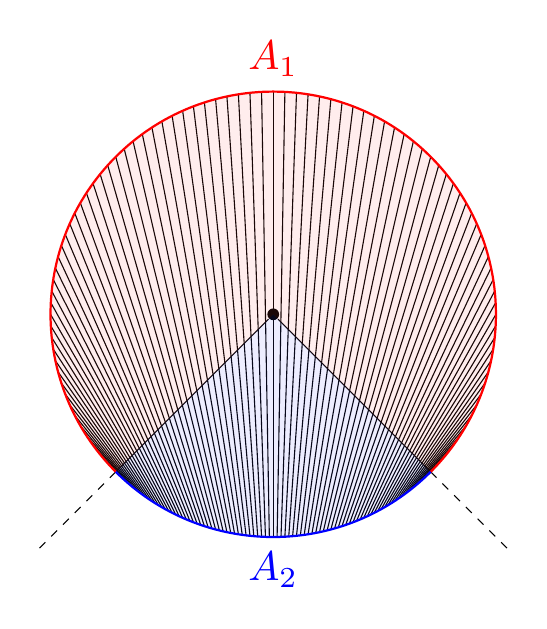
\begin{tikzpicture}[every node/.style={scale=1.5}]
  \node[fill=black, circle, inner sep=1pt] (x) at (0,0) {};

  % Radius of the ball
  \pgfmathsetmacro{\r}{2*sqrt(2)}

  % Draw the circle
  % \filldraw[fill=red!70!white, fill opacity=.1, draw=black] (x) circle
  % (\r);

  % Use a 45-45-90 triangle for the edges
  \coordinate (side1end) at (-2, -2);
  \coordinate (side2end) at (2, -2);

  \draw (side1end) -- (x) -- (side2end);

  % Extend them past our epsilon ball with dotted segments
  \coordinate (side1ext) at (-3, -3);
  \coordinate (side2ext) at (3, -3);

  \draw[dashed] (side1end) -- (side1ext);
  \draw[dashed] (side2end) -- (side2ext);

  % Iterate through theta values
  \foreach \t in {0, 1, ..., 90}{
    \pgfmathsetmacro{\tstart}{\t + 225}
    \pgfmathsetmacro{\tend}{225-3*\t}

    \pgfmathsetmacro{\xstart}{\r * cos(\tstart)}
    \pgfmathsetmacro{\ystart}{\r * sin(\tstart)}

    \pgfmathsetmacro{\xend}{\r * cos(\tend)}
    \pgfmathsetmacro{\yend}{\r * sin(\tend)}

    \draw[thin] (\xstart, \ystart) -- (\xend, \yend);
  }

  \fill[red!70!white, opacity=.1] (side2end) arc (-45:225:\r) -- (0,0)
  -- (side2end);
  \draw[red, thick] (2, -2) arc(-45:225:\r) node[midway, above] {$A_1$};
  % \node[red] () at (0, 1.5) {$R_1$};

  \fill[blue!70!white, opacity=.1] (side1end) -- (0,0) -- (side2end)
  arc (315:225:\r) --cycle;
  \draw[blue, thick] (-2, -2) arc(225:315:\r) node[midway, below] {$A_2$};
  % \node[blue] () at (0, -1.5) {$R_2$};


  % \fill[red,name intersections={of=line 1 and line 2,total=\t}]
  %   \foreach \s in {1,...,\t}{(intersection-\s) circle (2pt) node {\footnotesize\s}};



\end{tikzpicture}
\end{document}
